\chapter{Evaluation}
\label{sect:eval_intro}
	We evaluated our runtime's implementation performance by running some microbenchmark applications and
three small applications (fibonacci, quicksort, LU).  We run all benchmarks on two Intel(R) Xeon(R) 
CPU E5645@2.40GHz with with 6 available cores on each machine, totaling to 12 cores connected through 
a network socket. We have compiled the runtime and application code using g++ version 4.6.3 with 
level 3 optimizations enabled.  For the MPI library we used OpenMPI version 1.4.3.

\section{Microbenchmarks}
\label{sect:microbenchmark}
	Our first microbenchmark is a ping pong application, which is used to measure the time needed to send a 
message from the master to a worker node and the time needed for the worker node to respond back to the master.
Using the future interface, the master simply calls async with a functor that takes a string argument ("ping") 
and returns only a string value ("pong"), without doing any other computations in the functor's body.  We run
the ping pong microbenchmark using the configuration described in~\ref{sect:eval_intro} and the message was 
received by the master in 0.8ms.


	The rest of our microbenchmarks, aim to help us understand better the time needed to issue a job from one
node to another.  To achieve this, we designed one microbenchmark application, where the master node issues
a functor, with only a return statement in his body, which takes a variable number of arguments, each argument
can be either a scalar value or a vector container.  In figure~\ref{fig:issue_time_scalar_vs_containers} we report
the time needed to issue a job that takes a variable number of scalar arguments comparing it with the time needed
to issue a variable number of vector objects of one element.  Although the vector object arguments are more complex
to serialize, we see that the difference in execution time is marginal.  Moreover, we see that the number of arguments
has that need to be transfered, have minimal implact on execution time.  
Figure~\ref{fig:issue_time_different_argnum_same_size} shows the execution time of issuing functor objects with different
vector argument sizes.  In all cases the total number of elements totals to 1200000 (e.g. 1 vector of 1200000 elements or
4 vectors of 300000 elements).   The numbers reported are the median values of 20 runs, and by manual observation 
we can verify that the numbers have been consistent.
As of now, we have no insight as to why having 2 vector objects is more cost efficient
than having only one and the differences cannot be considered "noise". In figure~\ref{fig:job_issue_time_different_argsizes}
we can observe how the size of the arguments can affect execution time.  We see that the size of the arguments (here the 
size of 1 vector object) can exponentially increase execution time.  As expected, the size of the arguments is the factor
that can influence performance the most.

\begin{figure}[!ht]
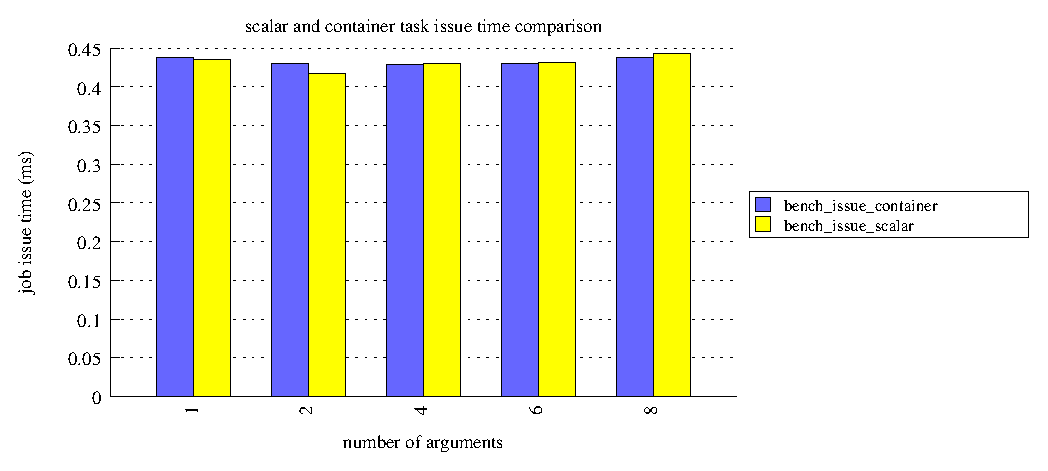
\includegraphics[width=\columnwidth]{figures/job_issue_time_scalar_vs_container_bars}
\caption{Comparison between issuing functors with scalar arguments versus vector objects of size 1}
\label{fig:issue_time_scalar_vs_containers}
\end{figure}

\begin{figure}[!ht]
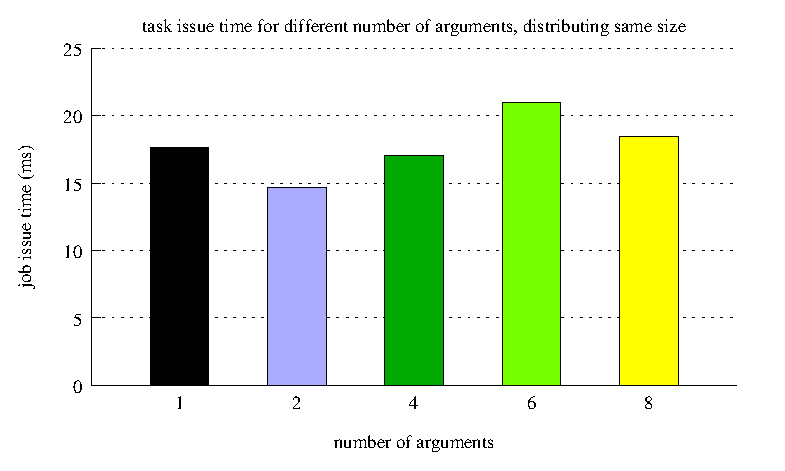
\includegraphics[width=\columnwidth]{figures/job_issue_time_different_argnums_same_size_bars}
\caption{Comparison between issuing functors with different number of vector arguments, but total 
				size of arguments is the same in all cases.}
\label{fig:issue_time_different_argnum_same_size}
\end{figure}

\begin{figure}[!ht]
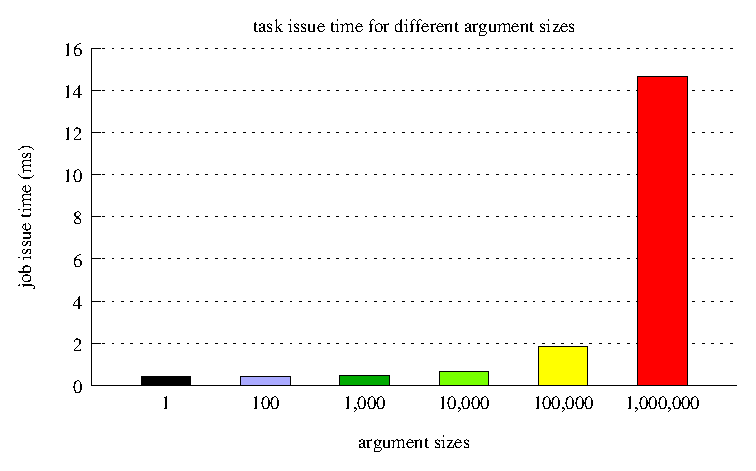
\includegraphics[width=\columnwidth]{figures/job_issue_time_different_argsizes}
\caption{Comparison between issuing functors with 1 vector argument of different sizes}
\label{fig:job_issue_time_different_argsizes}
\end{figure}

\section{Real Application Benchmarking}
\label{sect:real_app}
	In order to evaluate our runtime's performance we have implemented three algorithms using our future's interface.
\\
\\
	\textbf{Fibonacci}:  This is a simple implementation of the fibonacci function.  Figure~\ref{lst:fib} shows 
our implementation.  This recursive version is ideal to demonstrate the ease of use of the future's interface,
but the problem itself is of little interest on a distributed platform, since there is too little work to be 
done on each function.  Nevertheless, we include it in our results.  In our experiments we compute the fibonacci
sequence of 15.
\\
\\
	\textbf{Quicksort}:  Figure~\ref{lst:quicksort} shows our implementation.  The \emph{QsSequantial} 
function itself is a pretty standard
implementation of the common quicksort algorithm.  Parallelization is extracted at the \emph{quicksort} function, where the 
original array is partitioned and asynchrous quicksort functions are called until the \emph{min\_unit} value of elements
is reached, where from that point on the sequential version of the quicksort algorithm is called on each partition.
Notice that for the asynchronous branch of the code, we need to copy each partition in order to send it over the worker 
process and also merge the results of the async functions into the original array.  This additional overhead along with 
the communication overhead makes it necessary to sort small sub arrays sequentially.  For our experiments we sort an 
array of 100,000 doubles. 
\\
\\
	\textbf{Tiled LU}: We have implemented an LU factorization kernel using the Tiled LU algorithm as described in
~\cite{Buttari:2009:CPT:1486274.1486415}.  Figure~\ref(lst:tiledLUseq) shows a simplified version of the tiled
LU algorithm written in C++ style. All arrays are organized in tiles, each tile is a smaller sub array.  Array
\emph{A} is the input array.  In the first step an LU factorization is run on tile \emph{A[k][k]} (\emph{dgetrf} 
function).  The resulting arrays are the lower triangular \emph{L}, the upper triangular \emph{U}, both of which 
are stored in \emph{A[k][k]}, and the transmutation matrix \emph{P[k][k]}.  
The \emph{dgessm} function applies the \emph{L} and 
\emph{U} transformations on all tiles on row k, updating tiles \emph{L[k][k...TOTAL\_TILES]}. \emph{dtstrf}
function performs a block LU factorization on the array formed by coupling the upper triangular part of
\emph{A[k][k]} with \emph{A[k][k]}.
This function returns an upper triangular array, stored in \emph{A[k][k]}, a lower triangular array 
stored in \emph{A[m][k]} and a permutation array P[m][k].  The \emph{dssss} function updates the subarray
formed by tiles \emph{A[k+1...TOTAL\_TILES][k+1...TOTAL\_TILES]} by applying the  transformation computed by \emph{dtstrf}
of the coupled array of the upper triangular part of emph{A[k][n]} and array emph{A[m][n]}.  For the kernels \emph{dgetrf},
\emph{dgessm}, \emph{dtstrf} and \emph{dssssm}, we use the implementation found in the Plasma project
~\cite{1742-6596-180-1-012037} 

	
	Figure~\ref{lst:tiledLUpar} shows a simplified version of our parallel implementation.  The master process 
starts by executing the \emph{dgetrf}  function.  As soon as it completes, we can apply 
the \emph{dgessm} function on the rest of the tiles on row k (k being the step index we are currenlty working on).
Function \emph{dgessm} only requires the L and U factors from \emph{dgetrf} applied on A[k][k], thus we can issue them 
asynchronously, since all dependencies are met
We use here a special array of futures \emph{fA} to hold the return value \emph{dgessm}.   
Next, we apply the blocking LU transformation (\emph{dtstrf}) on the rest of the tiles on column k.  Here, because
each \emph{dtstrf} requires the updated A[k][k] tile from the previous application of \emph{dtstrf}, we cannot issue
them in asynchronously.  Instead, after running a \emph{dtstrf} we immediately issue asynchronous calls to \emph{dssssm}.
This function needs to wait from the \emph{dtstrf} that is applied on the first tile on the row, for the \emph{dgessm}
function that will be applied on the first tile of the column, and from the previous, if any, application of \emph{dgessssm}
on the tile just above the current one, that \emph{dgessssm} is applied.  Because \emph{dssssm} modifies two arrays, we use
a struct to represent the coupling of tile A and the upper triangular array U.  The variable cpldAU, is an array of futures
of that struct type.  The parallelization strategy described, allows us to work on each column asynchronously.  

\begin{figure}[!ht]
\begin{lstlisting}
/* a sequential qs */
void QsSequential(vector<double>& array, const long left, const long right){
    if(left < right){
        const long part = QsPartition(array, left, right);
        QsSequential(array,part + 1,right);
        QsSequential(array,left,part - 1);
    }
}
 
/** A task dispatcher */
class quicksort {
public:
	quicksort() {};
	~quicksort() {};
	vector<double> operator()(vector<double> array, const int deep) {
		const int left = 0;
		const int right = array.size()-1;
    if(left < right){
        if(array.size() > min_unit) {
            const long part = QsPartition(array, left, right);
 						vector<double> subarrA((right)-(part+1)+1), subarrB(part-1-left+1);
						Copy(subarrA, array, part+1, right+1);
						Copy(subarrB, array, left, part);
						quicksort qsort;
						future<vector<double> > res1, res2;
						res1 = async2(subarrA.size(), qsort, subarrA, deep-1);
						res2 = async2(subarrB.size(), qsort, subarrB, deep-1);
            subarrA = res1.get();
            subarrB = res2.get();
						Merge(array, subarrB, subarrA);
        }
        else {
            const long part = QsPartition(array, left, right);
            QsSequential(array,part + 1,right);
            QsSequential(array,left,part - 1);
        }
    }
		return array;
	}
};

\end{lstlisting}
\caption{A quicksort implementation using the distributed futures interface}
\label{lst:quicksort}
\end{figure}


\begin{figure}[!ht]
\begin{lstlisting}
for(int k = 0; k < TOTAL_TILES; k++) {
	dgetrf(A[k][k], P[k][k]);
	for(int n = k+1; n < TOTAL_TILES; n++) {
		dgessm(A[k][n], A[k][k], P[k][k])
	}
  for(int m = k+1; m < TOTAL_TILES; m++) {
		dtstrf(A[k][k], A[m][k] , P[m][k]);
  	for(int n=k+1; n < TOTAL_TILES; n++) {
			dssssm(U[k][n], A[m][n], L[m][k], A[m][k], P[m][k]);
		}
	}
}

\end{lstlisting}
\caption{The tiled LU kernel implementation}
\label{lst:tiledLUseq}
\end{figure}


\begin{figure}[!ht]
\begin{lstlisting}
for(int k = 0; k < TOTAL_TILES; k++) {
	A[k][k] = cpldAU[k][k].get().A;
	dgetrf(A[k][k], P[k][k]);
	for(int n = k+1; n < TOTAL_TILES; n++) {
		A[k][n] = cpldAU[k][n].get().A;
		fA[k][n] = async(dgessm, A[k][n], A[k][k], P[k][k]);
	}
  for(int m = k+1; m < TOTAL_TILES; m++) {
		A[m][k] = cpldAU.get().A;
		dtstrf(A[k][k], A[m][k].get() , P[m][k]);
  	for(int n=k+1; n < TOTAL_TILES; n++) {
			if(m == k+1)
				A[k][n] = fA[k][n].get();
			else
				A[k][n] = cpldAU.get().U;
			A[m][n] = cpldAU.get().A;
			cpldAU[m][n] = async(dssssm, A[k][n], A[m][n], L[m][k], A[m][k], P[m][k]);
		}
	}
}

\end{lstlisting}
\caption{The tiled LU parallel kernel implementation}
\label{lst:tiledLUpar}
\end{figure}

	In figure~\ref{fig:apps_scalability} we report the execution times for running the three applications on the
machine setup we described in section~\ref{sect:eval_intro}.  We measure only the algorithm and no initialization
and finalization times of the runtime system, etc.
We observe that we do not manage to get any speedup on 
any application, on the contrary we get a slowdown (figure~\ref{fig:apps_speedup}).
There is some improvement as we increase the cores for 
the fibonacci and quicksort applications, but in no case we manage to even match the sequential problem.  In 
figure~\ref{fig:apps_breakdowns_6cores} 
we show the breakdowns for the master application and the slaves, for running the applications on 6 cores.
\emph{Job issue time} is the time needed to send a \emph{job} from one process to another. This time includes
time spend in the scheduler, to find the next worker and time spend on serialization of the \emph{job} object
and sending it to the worker.  \emph{Job execution time} is the time spent on running the actual code of the
\emph{job} that was issued via an async call.  \emph{User code time} is the time the master process spends
running code that is not related with the runtime.  \emph{Idle time} is time spend waiting to retrieve a future 
value and for the workers, it's also time spent waiting for a \emph{job} to become available in their stacks.
\emph{Rest of time} is the rest of the overhead that is imposed by the runtime.  This time can be for example 
the time needed to send the return value of the asynchronous execution of a \emph{job} by a worker.  In all 
applications we see that the either \emph{job issue time} or \emph{rest of time} are the greatest sources of 
overhead, while a fair amount of time is also spent on \emph{idle time}.  These overhead times are too great
compared to the actual work done by any of the processes, so small problems and kernels are not fit to be 
run on our runtime system, as the current implementation stands.  At this stage it is unclear whether the issue
is the MPI library or the implementation.  We will further investigate the current issues.  Moreover, figure
~\ref{fig:app_breakdowns_w_init} shows the same breakdowns with figure~\ref{fig:app_breakdowns_6cores}, with 
the addition of initialization and finalization times.  The initialization and finalization include the 
creation and finalization of the communication module (in our experiments that's MPI), creation and destruction
of the shared memory (MPI Windows) and scheduler.  The initialization time is constant on all applications, since
it mainly depends on the number of processes, while the finalization time is negligible. 

\begin{figure}[!ht]
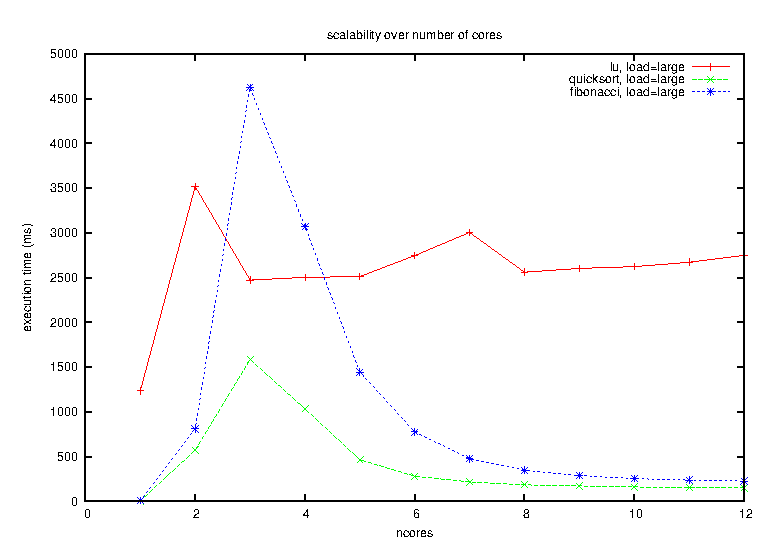
\includegraphics[width=\columnwidth]{figures/apps_scalability}
\caption{Scalability graph for fibonacci, quicksort and LU}
\label{fig:apps_scalability}
\end{figure}

\begin{figure}[!ht]
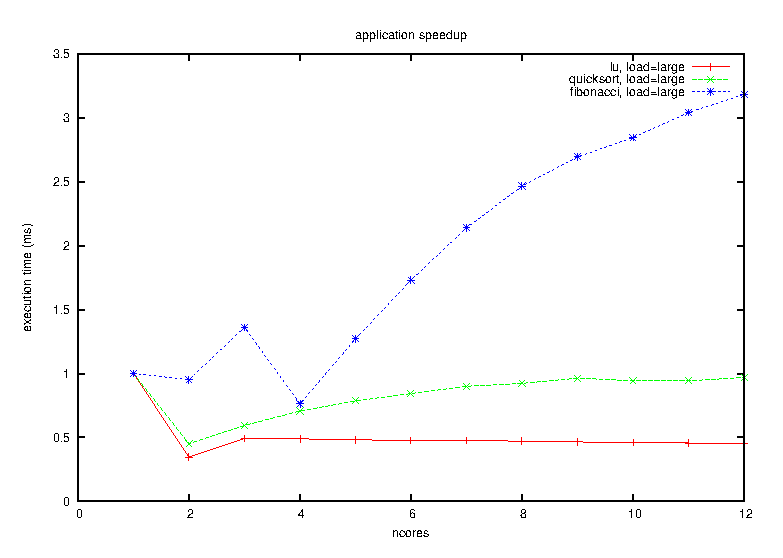
\includegraphics[width=\columnwidth]{figures/apps_speedup}
\caption{Speedup graph for fibonacci, quicksort and LU}
\label{fig:apps_speedup}
\end{figure}

\begin{figure}[!ht]
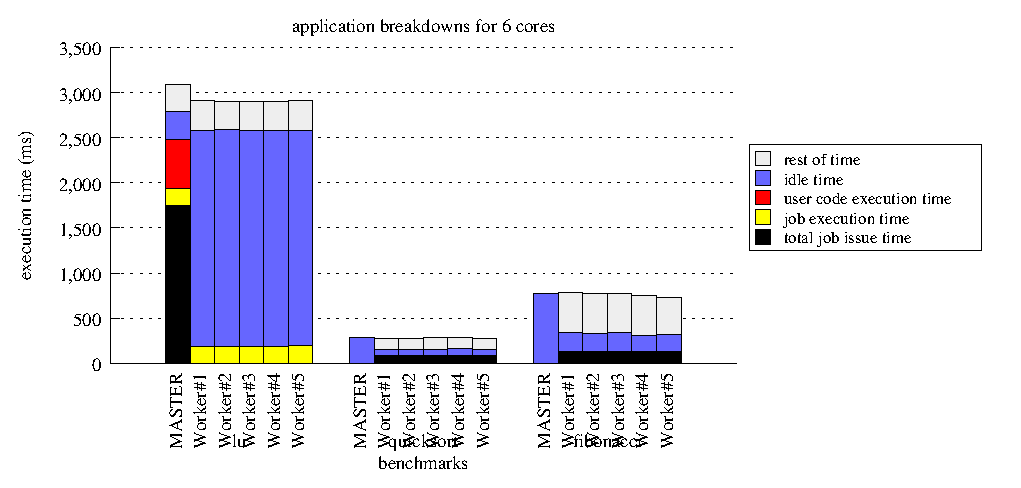
\includegraphics[width=\columnwidth]{figures/app_breakdowns_6cores}
\caption{Breakdowns of master and worker execution time graph for fibonacci, quicksort and LU}
\label{fig:app_breakdowns_6cores}
\end{figure}

\begin{figure}[!ht]
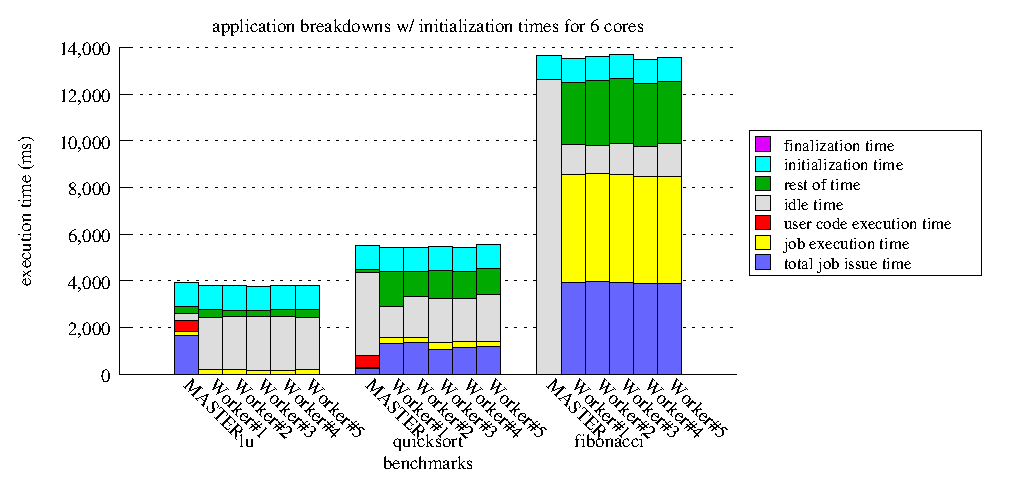
\includegraphics[width=\columnwidth]{figures/app_breakdowns_w_init}
\caption{Breakdowns of master and worker execution time graph for fibonacci, quicksort and LU, with initialization
and finalization times}
\label{fig:app_breakdowns_w_init}
\end{figure}



